%% EcoPE-GAT manuscript (Elsevier cas-sc, single column), rebuilt 2026-11-16.
%% Every number below comes from results/numbers.tex, generated by src/07_tables.py.
%% Text marked \pending{...} (red) is waiting for results of the running experiments.
\PassOptionsToPackage{hyperfootnotes=false}{hyperref}
\documentclass[a4paper,fleqn]{cas-sc}

\usepackage[authoryear]{natbib}
\RenewDocumentCommand \printorcid { } { }
\usepackage{amsmath,amssymb}
\usepackage{booktabs}
\usepackage{enumitem}
\usepackage{graphicx}
\usepackage{xcolor}
\usepackage{placeins}

% AUTO-GENERATED by src/07_tables.py -- do not edit by hand.

\newcommand{\nPlotsTotal}{95{,}104}  % sPlotOpen plots
\newcommand{\nPlotsNoDate}{15{,}019}
\newcommand{\surveyYearMin}{1888}
\newcommand{\surveyYearMax}{2015}
\newcommand{\pctPlotsPreNineteen}{44}  % dated plots surveyed before 1999 (%)
\newcommand{\nEligible}{44{,}772}
\newcommand{\nEligibleCoords}{41{,}132}
\newcommand{\nEligibleDatasets}{93}
\newcommand{\gbifRecordsRaw}{22{,}129}
\newcommand{\gbifSpecies}{27}
\newcommand{\gbifPresent}{21{,}674}
\newcommand{\gbifUncOK}{21{,}468}
\newcommand{\gbifNoMS}{9{,}926}
\newcommand{\gbifFinal}{8{,}276}  % main variant after dedup
\newcommand{\gbifFinalAllBasis}{11{,}475}
\newcommand{\gbifFinalUncDrop}{5{,}538}
\newcommand{\pctUncMissing}{71}
\newcommand{\pctMaterialSample}{54}
\newcommand{\nMaterialSample}{12{,}001}
\newcommand{\prevNfive}{5.0}  % % positive, main, N=5
\newcommand{\nPosNfive}{2{,}231}
\newcommand{\prevAllBasisNfive}{6.7}
\newcommand{\prevNseven}{6.7}  % % positive, main, N=7
\newcommand{\nPosNseven}{3{,}007}
\newcommand{\prevAllBasisNseven}{9.7}
\newcommand{\prevNonezero}{8.5}  % % positive, main, N=10
\newcommand{\nPosNonezero}{3{,}804}
\newcommand{\prevAllBasisNonezero}{12.9}
\newcommand{\pctPrior}{5.7}
\newcommand{\prevGivenPriorNfive}{43}
\newcommand{\prevGivenNoPriorNfive}{2.7}
\newcommand{\effortOutROCNfive}{0.88}  % effort outside label window
\newcommand{\effortOutPRNfive}{0.50}
\newcommand{\priorCountPRNfive}{0.31}  % prior count as score
\newcommand{\priorCountROCNfive}{0.73}
\newcommand{\prevGivenPriorNseven}{51}
\newcommand{\prevGivenNoPriorNseven}{4.0}
\newcommand{\effortOutROCNseven}{0.86}  % effort outside label window
\newcommand{\effortOutPRNseven}{0.56}
\newcommand{\priorCountPRNseven}{0.32}  % prior count as score
\newcommand{\priorCountROCNseven}{0.70}
\newcommand{\prevGivenPriorNonezero}{57}
\newcommand{\prevGivenNoPriorNonezero}{5.5}
\newcommand{\effortOutROCNonezero}{0.81}  % effort outside label window
\newcommand{\effortOutPRNonezero}{0.51}
\newcommand{\priorCountPRNonezero}{0.32}  % prior count as score
\newcommand{\priorCountROCNonezero}{0.68}
\newcommand{\prevContNonezeroEurope}{26.4}
\newcommand{\prevContNonezeroNorthAmerica}{1.4}
\newcommand{\prevContNonezeroOceania}{13.9}
\newcommand{\nBlocks}{270}
\newcommand{\blockKm}{500}
\newcommand{\foldSizeMin}{8{,}933}
\newcommand{\foldSizeMax}{8{,}997}
\newcommand{\nFolds}{5}
\newcommand{\nSeeds}{5}
\newcommand{\nTrials}{30}
\newcommand{\tuningHorizon}{10}
\newcommand{\bufferKm}{50}
\newcommand{\kNeighbours}{10}

\newcommand{\pending}[1]{\textcolor{red}{[PENDING: #1]}}

\begin{document}
\let\WriteBookmarks\relax
\def\floatpagepagefraction{1}
\def\textpagefraction{.001}

\shorttitle{EcoPE-GAT}
\shortauthors{Laib and Laiche}

% Title to be revisited once the results are in (see the paper <-> code report).
\title[mode=title]{EcoPE-GAT: Graph Attention Networks with Ecological Positional Encoding for Global Plant Pathogen Emergence Prediction}

\author[1]{Mohamed Djounaid Laib}
\ead{Mohamed.djounaid.laib_d@usthb.edu.dz}
\credit{Conceptualization, Methodology, Software, Formal analysis, Writing -- original draft}

\author[1,2]{Nacéra Laiche}
\cormark[1]
\ead{nlaiche@usthb.dz}
\credit{Supervision, Methodology, Writing -- review \& editing}

\affiliation[1]{organization={LRIA, University of Sciences and Technology Houari Boumediene (USTHB)},
            city={Algiers},
            country={Algeria}}

\affiliation[2]{organization={Faculty of Computer Science, Artificial Intelligence and Data Sciences Department, University of Sciences and Technology Houari Boumediene (USTHB)},
            city={Algiers},
            country={Algeria}}

\cortext[1]{Corresponding author}

\begin{abstract}
\pending{Abstract ($\leq$150 words) to be written from the final results: task and data (\nEligible{} sPlotOpen plots, GBIF download, horizons 5/7/10 years); evaluation design (spatially blocked CV, transductive vs inductive, prior-presence and effort baselines); main quantitative findings with uncertainty; what the comparison implies about when graph models help.}
\end{abstract}

\begin{highlights}
\item \pending{3--5 highlights, each $\leq$85 characters, written from the final results.}
\end{highlights}

\begin{keywords}
Graph neural network \sep Positional encoding \sep Plant pathogens \sep Functional traits \sep Spatial cross-validation \sep Sampling bias \sep Model evaluation
\end{keywords}

\maketitle

% =========================================================
\section{Introduction}
\label{sec:intro}

Plant pathogens are a pervasive and poorly predicted threat to terrestrial ecosystems and food security \citep{bebber2014,fisher2012}. Large open databases now describe both sides of the host--pathogen relationship at global scale: vegetation-plot databases such as sPlotOpen characterise the functional composition of tens of thousands of plant communities \citep{sabatini2021}, and the Global Biodiversity Information Facility (GBIF) aggregates millions of georeferenced occurrence records, including records of plant pathogens. Whether the functional composition of a plant community carries information about where pathogens will be reported next is an open question at this scale.

Two properties of these data make the question harder than it looks. First, plots are not independent observations: communities with similar functional profiles may share susceptibility, and nearby plots share environment, survey campaign and reporting intensity. Graph neural networks (GNNs) offer a way to model such dependence explicitly, by passing information between related plots \citep{kipf2017,hamilton2017,velickovic2018}. Second, occurrence records reflect where people look as much as where organisms occur \citep{beck2014,phillips2009}. A model that predicts future records may therefore learn surveillance effort rather than ecological risk, and evaluation designs that ignore spatial structure can overstate how well it generalises \citep{roberts2017,ploton2020}.

In this paper we formulate the prediction of future pathogen records near vegetation plots as node classification on a graph that connects plots by similarity in functional-trait space, and we propose EcoPE, an ecological positional encoding that injects climate, location and biome context into a graph attention network (EcoPE-GAT). We then evaluate this model, and the question of whether graph structure helps at all, under a protocol designed to expose the confounds described above: spatially blocked cross-validation, transductive and inductive graph settings, strong tabular baselines with identical tuning budgets, and explicit baselines for prior presence of the pathogen and for sampling effort.

Our contributions are:
\begin{enumerate}[leftmargin=1.4em]
  \item A reproducible global dataset linking \nEligible{} sPlotOpen plots to a single citable GBIF download of \gbifSpecies{} plant-pathogen species, with labels restricted to plots whose whole prediction window lies inside the GBIF coverage, and with prior-presence and sampling-effort covariates.
  \item EcoPE-GAT, and a set of controls that isolate what it adds: a plain GAT, a GAT receiving the same context variables by direct concatenation, GCN and GraphSAGE, and a hybrid gradient-boosting model using graph-neighbourhood labels.
  \item A comparison of transductive and inductive graph training under spatially blocked cross-validation, which tests directly whether test nodes present in the graph during training affect apparent generalisation.
  \item An assessment of how much of the predictive signal is attributable to prior pathogen presence and to sampling effort rather than to community traits. \pending{one-sentence summary of the answer}
\end{enumerate}

Section~\ref{sec:relwork} reviews related work. Section~\ref{sec:data} describes the data and labels, Section~\ref{sec:models} the models, and Section~\ref{sec:protocol} the evaluation protocol. Results are reported in Section~\ref{sec:results} and discussed in Section~\ref{sec:discussion}.

% =========================================================
\section{Related work}
\label{sec:relwork}

\subsection{Functional traits and plant disease}

Plant functional traits are measurable characteristics of species, such as leaf area, specific leaf area or leaf nitrogen content, that influence growth, survival and reproduction. Aggregated as community-weighted means (CWM) and variances (CWV), they give a compact, taxonomy-independent description of a community's ecological strategy \citep{lavorel2002}, and they vary systematically with environment at global scale \citep{bruelheide2018}. Host traits influence responses to pathogens at the individual level \citep{jin2021}, and host community traits shape disease risk along environmental gradients \citep{halliday2021}. Correlative species distribution models are the standard tool for macroecological prediction, including of plant disease \citep{elith2009}, but their transferability beyond the conditions they were fitted on remains a concern \citep{guillera2015}. Representation-learning alternatives to traits have also been proposed, for instance species embeddings learned from co-occurrence in sPlotOpen \citep{siefert2024}. We are not aware of work that uses community traits from vegetation plots as predictors of future pathogen records at global scale.

\subsection{Graph neural networks in ecology}

Gradient-boosted trees and random forests are strong baselines for tabular ecological data \citep{valavi2022} and often outperform deep learning on tabular benchmarks \citep{grinsztajn2022}. GNNs add a mechanism for exploiting relations between observations: GCN aggregates neighbours with fixed normalised weights \citep{kipf2017}, GraphSAGE learns aggregation functions that apply to unseen nodes \citep{hamilton2017}, and GAT learns per-edge attention coefficients \citep{velickovic2018}. GNNs have recently been applied to species distribution modelling, using graphs of landscape patches \citep{wu2025} or heterogeneous species--location graphs \citep{harrell2025}, with performance comparable to or better than conventional baselines in those settings. These graphs are defined by spatial proximity or species--location relations; graphs of vegetation plots defined by functional-trait similarity have, to our knowledge, not been studied.

\subsection{Positional encodings for graphs}

Positional encodings give GNN nodes information that message passing alone cannot recover. Laplacian eigenvectors \citep{dwivedi2020} and distance encodings \citep{li2020} describe a node's position in the graph topology. For geographic data, PE-GNN learns an encoding of raw coordinates and uses it with a spatial-proximity graph \citep{klemmer2023pegnn}; a related encoder has been used for soil organic carbon estimation \citep{zhao2023}. EcoPE differs in that it encodes ecological context (climate, location and biome) for a graph whose edges are not geographic. Whether a dedicated encoder adds anything over simply concatenating the same variables to the node features is an empirical question that we test directly.

\subsection{Sampling bias and spatial evaluation}

Occurrence data are geographically biased towards well-surveyed regions \citep{beck2014}, and presence-only models absorb this bias unless it is modelled, for example through target-group background data \citep{phillips2009}. When observations are spatially autocorrelated, random cross-validation overestimates predictive performance; spatially blocked designs give more realistic estimates \citep{roberts2017,valavi2019,ploton2020}. Graph models add a further subtlety: in transductive training, test nodes are present in the graph and their features influence training-node representations, whereas in inductive training they are not. GNN studies on spatio-temporal ecological or epidemiological data are commonly evaluated transductively \citep[e.g.][]{croft2023}, and the effect of this choice on spatial generalisation estimates is rarely quantified.

% =========================================================
\section{Data}
\label{sec:data}

\subsection{Vegetation plots}

We used sPlotOpen \citep{sabatini2021,splotdata}, which contains \nPlotsTotal{} vegetation plots surveyed between \surveyYearMin{} and \surveyYearMax{}. For each plot we used the community-weighted mean and variance of 18 functional traits (36 variables), species richness, the two trait-coverage indices provided with the data, the two soil--climate principal components (SoilClim PC1 and PC2), latitude, longitude, biome (ten zones) and survey date. Survey year was parsed from the recording date; \nPlotsNoDate{} plots without a date were excluded.

\subsection{Pathogen records}

Pathogen occurrences come from a single GBIF download of \gbifRecordsRaw{} records of \gbifSpecies{} plant-pathogen species recorded between 2000 and 2025 \citep{gbifdownload}. Filters were applied in the following order, and record counts per species after each step are given in Table~S1: (i) occurrenceStatus equal to PRESENT (\gbifPresent{} records remaining); (ii) year within 2000--2025 and valid, non-zero coordinates; (iii) coordinate uncertainty at most 10~km (\gbifUncOK{} remaining). Coordinate uncertainty was missing for \pctUncMissing\% of the raw records; in the main analysis these records were kept, and dropping them is a sensitivity analysis. (iv) Records with basisOfRecord equal to MATERIAL\_SAMPLE were removed (\gbifNoMS{} remaining). These \nMaterialSample{} records (\pctMaterialSample\% of the download) come mostly from environmental-DNA datasets (soil, air and marine metabarcoding and sequence repositories); they document the presence of the organism's DNA rather than a reported occurrence on plants, and keeping them is a sensitivity analysis. (v) Duplicates, defined as the same species at the same coordinates rounded to 0.01\textdegree{} in the same year, were removed, leaving \gbifFinal{} records for the main analysis.

\subsection{Spatial join and labels}

Plots and records were joined by great-circle (haversine) distance using a ball tree. Let $r_i$ be the survey year of plot $i$ and $\mathcal{B}_i$ the set of filtered records within $\bufferKm$~km of the plot. The label for horizon $N$ is
\begin{equation}
y_i^{(N)} = \mathbb{1}\left[\exists\, j \in \mathcal{B}_i : 0 < t_j - r_i \leq N\right],
\label{eq:label}
\end{equation}
where $t_j$ is the year of record $j$, and $N \in \{5, 7, 10\}$ years. Because GBIF coverage starts in 2000, a plot can only be labelled if its whole window $(r_i, r_i+N]$ lies within 2000--2025, that is, $r_i \geq 1999$ and $r_i + N \leq 2025$. This excludes the \pctPlotsPreNineteen\% of dated plots surveyed before 1999, which could never be positive and would otherwise allow a model to learn the survey period of a dataset instead of pathogen risk. Since the latest sPlotOpen survey is from \surveyYearMax, the upper bound never binds and the same \nEligible{} plots (\nEligibleCoords{} distinct locations from \nEligibleDatasets{} source datasets) are labelled for all three horizons. Records from the survey year itself are used neither for the label nor as prior presence. Buffers of 25 and 100~km are used as sensitivity analyses.

The positive class comprises \prevNfive\%, \prevNseven\% and \prevNonezero\% of eligible plots at $N = 5$, 7 and 10 (\nPosNfive, \nPosNseven{} and \nPosNonezero{} plots). Prevalence is strongly structured geographically: at $N=10$ it is \prevContNonezeroEurope\% in Europe, \prevContNonezeroOceania\% in Oceania and \prevContNonezeroNorthAmerica\% in North America (Figures~S1--S4).

\subsection{Prior presence and sampling effort}

For each plot we counted the filtered records within the buffer strictly before the survey year (prior presence), and the number of distinct species among them. These quantities are available at prediction time and are used both as a baseline and as features (feature set C, Section~\ref{sec:features}). \pctPrior\% of eligible plots have at least one prior record; among them \prevGivenPriorNfive\% are positive at $N=5$, against \prevGivenNoPriorNfive\% among plots without a prior record. Because the download starts in 2000, the look-back window for prior presence grows with survey year, from zero years for plots surveyed in 1999 to fifteen years for plots surveyed in 2015.

As a proxy for sampling effort we used target-group counts \citep{phillips2009}: the number of records of the \gbifSpecies{} species within the buffer in all years outside the label window. This proxy is built from the same records as the label and uses future years, so it is not a usable predictor and is not independent of the outcome; we use it only as a diagnostic of how much of the label can be ranked by surveillance intensity alone. Used directly as a score, it reaches a ROC-AUC of \effortOutROCNfive{} (PR-AUC \effortOutPRNfive) at $N=5$, without any model fitting.

% =========================================================
\section{Models}
\label{sec:models}

\subsection{Feature sets and preprocessing}
\label{sec:features}

We used three nested feature sets: (A) the 36 trait CWM and CWV variables, species richness and the two trait-coverage indices; (B) A plus ecological context, namely SoilClim PC1 and PC2, latitude, longitude and a one-hot encoding of biome; (C) B plus prior presence ($\log(1+\text{count})$ of prior records, number of prior species, and an indicator of any prior record). CWV variables and species richness were $\log(1+x)$-transformed. Within each training fold, missing values were imputed with the training median, a binary missingness indicator was added for every variable with missing training values, and all variables were standardised with training-fold statistics.

\subsection{Tabular models}

Logistic regression (L2-penalised), random forest \citep{breiman2001} with 300 trees, LightGBM gradient boosting \citep{ke2017} with up to 2{,}000 rounds and early stopping after 50 rounds on the inner validation set, and a multilayer perceptron (MLP) were trained on each feature set using scikit-learn \citep{pedregosa2011}, LightGBM and PyTorch \citep{paszke2019}. The MLP has one to three hidden layers, each with a linear layer, layer normalisation, GELU activation and dropout, with widths halving from the first layer. As a non-learned baseline, plots were ranked by their number of prior records.

\subsection{Trait-similarity graph}

Each plot is a node. Edges connect each plot to its $k = \kNeighbours$ nearest neighbours by Euclidean distance in the space of the 36 standardised trait variables (scaler fitted on the training fold), with edge weight $w_{ij} = 1/(1 + d_{ij})$. We built the graph in two ways. In the \emph{transductive} setting, the $k$-nearest-neighbour graph is computed over all nodes and symmetrised; test labels are hidden, but test features take part in message passing during training. In the \emph{inductive} setting, the graph among training nodes is built and symmetrised, and each inner-validation or test node receives directed edges from its $k$ nearest training nodes only. Held-out nodes therefore never send messages, so training-node representations are independent of held-out data. Values $k \in \{5, 20\}$ are a sensitivity analysis.

\subsection{Graph neural networks}

All graph models share the same structure, implemented in PyTorch Geometric \citep{fey2019}: an input projection (linear layer, layer normalisation, GELU) to a hidden width $h$; two graph layers with ELU activation and dropout; and a readout with one hidden layer of 64 units (ReLU) and a single output logit. We compared five variants.
\begin{itemize}[leftmargin=1.4em]
  \item \textbf{GCN} \citep{kipf2017}, with the edge weights $w_{ij}$ in the symmetric normalisation.
  \item \textbf{GraphSAGE} \citep{hamilton2017} with mean aggregation; this layer does not use edge weights.
  \item \textbf{GAT} \citep{velickovic2018} on feature set A. Each layer has $H$ heads of $h/H$ channels whose outputs are concatenated; the edge weight enters the attention score as an edge feature,
  \begin{equation}
  e_{ij} = \mathrm{LeakyReLU}\!\left(a^\top\left[W h_i \,\|\, W h_j \,\|\, W_e w_{ij}\right]\right), \qquad
  \alpha_{ij} = \frac{\exp(e_{ij})}{\sum_{l \in \mathcal{N}(i)} \exp(e_{il})},
  \end{equation}
  with dropout applied to the attention coefficients.
  \item \textbf{GAT + context}: the same GAT with the context variables of feature set B concatenated to the node features. This is the direct control for EcoPE.
  \item \textbf{EcoPE-GAT}: the GAT on feature set A, with the node features concatenated to an ecological positional encoding
  \begin{equation}
  p_i = f_\phi\!\left(\left[\text{PC1}_i, \text{PC2}_i, \phi_i, \lambda_i, \mathbf{b}_i\right]\right) \in \mathbb{R}^{32},
  \end{equation}
  where $\phi_i$ and $\lambda_i$ are latitude and longitude, $\mathbf{b}_i$ is the one-hot biome vector, and $f_\phi$ is a two-layer MLP (64 and 32 units, each followed by layer normalisation and GELU). The context variables are standardised with training-fold statistics.
\end{itemize}
Figure~\ref{fig:architecture} shows the EcoPE-GAT architecture.

\begin{figure}[pos=t]
  \centering
  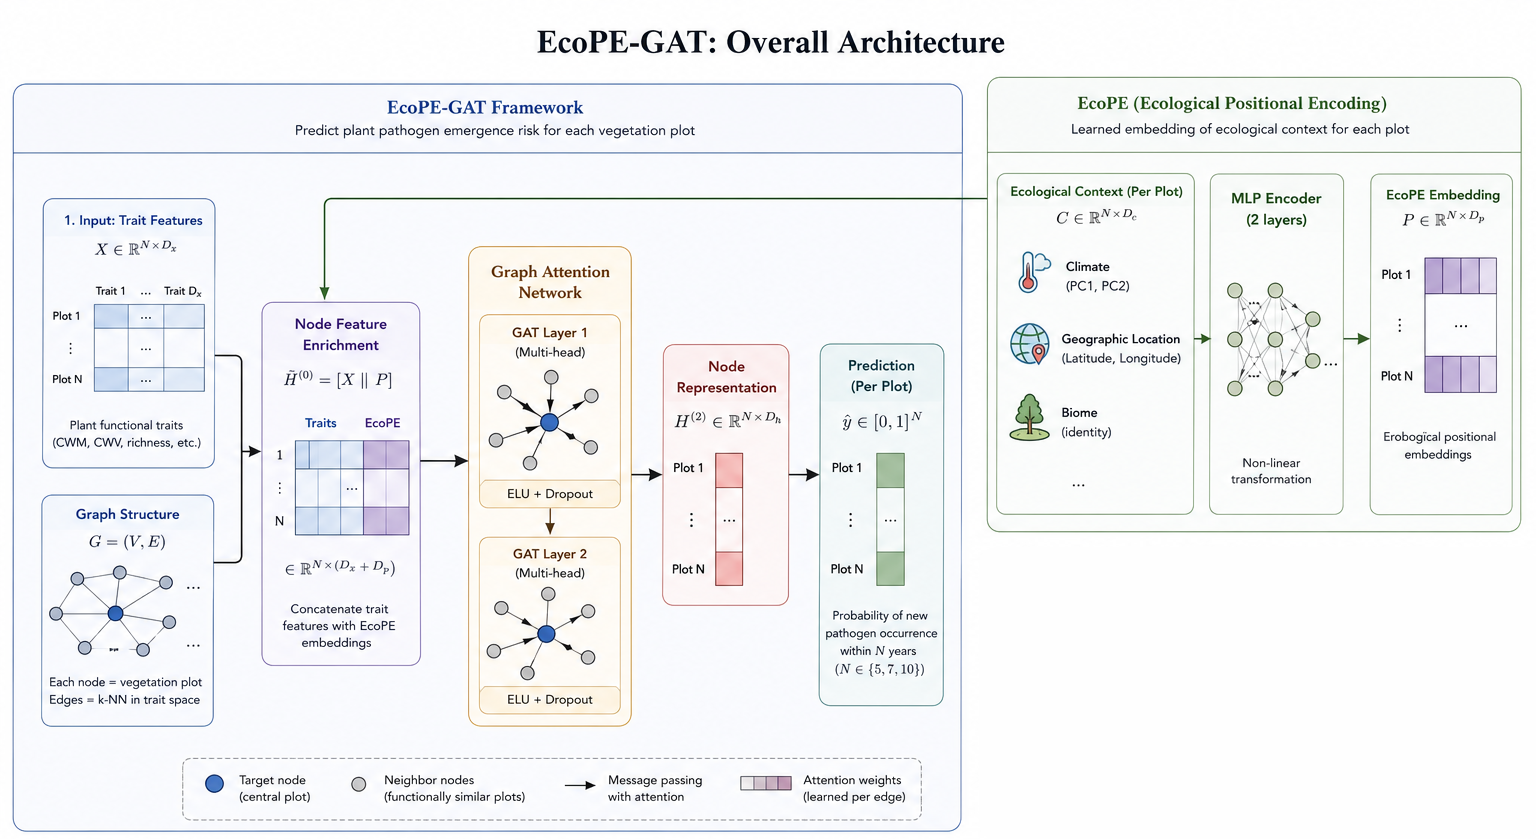
\includegraphics[width=\linewidth]{figures/ecope_gat_architecture.png}
  \caption{EcoPE-GAT. Trait features and the $k$-nearest-neighbour trait graph are combined with the EcoPE embedding of ecological context (climate principal components, location, biome) before two graph attention layers and an MLP readout produce the probability of a new pathogen record within $N$ years.}
  \label{fig:architecture}
\end{figure}

\subsection{Hybrid model}

The hybrid model is LightGBM on feature set B plus three graph-neighbourhood features computed from training labels only: the distance-weighted fraction of positive neighbours, the number of positive neighbours, and the mean distance to the $k$ nearest training plots in trait space. For inner-validation and test plots, neighbours are drawn from all training plots. For training plots the features are cross-fitted: training plots are split into five groups of spatial blocks, and each plot's neighbours are drawn only from the other groups. A training plot's own label, and the labels of plots from its own block, therefore never enter its features, which mimics the situation of a test plot in a held-out block.

\subsection{Training and hyperparameter tuning}

Neural models were trained by minimising binary cross-entropy, optionally with the positive class weighted by $n^-/n^+$ in the training set (a tuned option), using Adam \citep{kingma2015} with gradient clipping at norm 1.0. The learning rate was halved when the inner-validation PR-AUC had not improved for 10 epochs, and training stopped after 20 epochs without improvement (at most 200 epochs), restoring the best weights. Graph models were trained full-batch; the MLP used mini-batches of 2{,}048 plots.

Hyperparameters were tuned separately within every outer training fold with Optuna \citep{akiba2019} (TPE sampler), using the same budget of \nTrials{} trials for every model. Each trial was trained on the training part of the fold and scored by PR-AUC on the inner validation set (Section~\ref{sec:protocol}). To keep the computation feasible on a CPU workstation, tuning used the $N = \tuningHorizon$ labels, which have the most positives, and the selected hyperparameters were used for all three horizons within that fold. Graph models were tuned separately for the transductive and inductive settings. With the selected hyperparameters, each model was refitted with \nSeeds{} random seeds for each horizon and evaluated on the outer test fold. Search spaces are listed in Table~S2 and in the configuration file of the repository.

% =========================================================
\section{Evaluation protocol}
\label{sec:protocol}

\subsection{Cross-validation schemes}

The primary evaluation is spatially blocked five-fold cross-validation. Plots were assigned to blocks of approximately $\blockKm \times \blockKm$~km, defined by latitude bands of constant height and longitude intervals widened by $1/\cos(\text{latitude})$ so that cells have roughly constant area (\nBlocks{} occupied blocks). Blocks were assigned to five folds with stratification on the $N = 10$ label (\foldSizeMin--\foldSizeMax{} plots per fold), and the same folds were used for all horizons and models, so that comparisons are paired. Within each training fold, one fifth of the training blocks formed the inner validation set used for tuning and early stopping; it never overlaps the test fold or the remaining training blocks. As secondary schemes we used stratified random five-fold cross-validation (with a random inner validation set) and leave-one-continent-out cross-validation. \pending{report LOCO and random-CV results; note that Africa and South America have no positive plot at $N=5$, so PR-AUC is undefined for those held-out continents.}

\subsection{Metrics and statistical comparison}

The primary metric is PR-AUC (average precision), which is appropriate for imbalanced outcomes \citep{saito2015}; we also report ROC-AUC and the Brier score. The chance level of PR-AUC equals the prevalence of each test fold. Brier scores of models trained with class weighting are not calibrated and are reported for completeness. Results are given as mean $\pm$ standard deviation over the 25 fold--seed combinations. Models were compared with paired Wilcoxon signed-rank tests \citep{wilcoxon1945} over fold--seed combinations. \pending{bootstrap confidence intervals and multiple-comparison handling, as implemented in src/05\_analyses.py}

\subsection{Ablations and analyses}

\pending{describe exactly what src/05\_analyses.py implements: (i) EcoPE vs plain GAT vs GAT + context; (ii) removing each EcoPE input in turn; (iii) with and without prior presence; (iv) buffer 25/50/100~km and GBIF filtering variants; (v) $k \in \{5,10,20\}$; (vi) permutation importance or SHAP for the best tabular model and gradient-based attribution for the GNN; (vii) EcoPE embeddings coloured by variables that are not EcoPE inputs; (viii) enrichment of positives among top-5\% attention edges on test nodes only, with a 1{,}000-permutation test per horizon; (ix) error analysis by continent, biome, survey-year bin and source dataset; (x) within-dataset vs between-dataset performance.}

% =========================================================
\section{Results}
\label{sec:results}

\pending{All results sections are generated after the spatial-CV run completes. Planned content:
(1) Table 1: PR-AUC, ROC-AUC, Brier (mean $\pm$ sd) for every model and feature set, $N = 5, 7, 10$, spatial CV, with chance level;
(2) prior-presence and effort baselines vs learned models;
(3) EcoPE vs plain GAT vs GAT + context, with Wilcoxon $p$-values;
(4) transductive vs inductive;
(5) secondary schemes (random CV, leave-one-continent-out);
(6) ablations and sensitivity analyses;
(7) interpretation (feature importance, embeddings, attention enrichment with permutation tests);
(8) error analysis.}

% =========================================================
\section{Discussion}
\label{sec:discussion}

\pending{Written from the results. Points already established by the data analysis, to be developed:}

\subsection{What the labels measure}

The labels record whether a pathogen record was reported near a plot, not whether a pathogen emerged there. Their prevalence is dominated by geography and surveillance: a target-group effort count alone ranks plots with a ROC-AUC of \effortOutROCNfive{} at $N=5$, and positives are concentrated in a few regions and source datasets. Any model, tabular or graph-based, can reach high scores by recognising well-surveyed regions. \pending{relate to within-dataset vs between-dataset results.}

\subsection{When does graph structure help?}

\pending{Interpret graph vs tabular, EcoPE vs concatenation, transductive vs inductive, hybrid.}

\subsection{Limitations}

\begin{itemize}[leftmargin=1.4em]
  \item \textbf{Labels reflect reporting.} Labels are derived from occurrence records and confound pathogen presence with surveillance effort \citep{beck2014}. Our effort proxy uses the same \gbifSpecies{} species as the labels and is therefore not independent of them; an independent effort layer (for example all fungal records in GBIF) would allow a cleaner separation.
  \item \textbf{Species pool.} The download covers \gbifSpecies{} well-known pathogens, many of them crop pathogens; results may not transfer to pathogens of natural vegetation.
  \item \textbf{Temporal coverage.} Only plots surveyed from 1999 onwards can be labelled, which removes most historical plots. The look-back window for prior presence grows with survey year, so prior presence is partly confounded with survey period.
  \item \textbf{Missing uncertainty.} Most records lack a coordinate uncertainty value; keeping them may admit imprecise coordinates. The sensitivity analysis without them is reported in Section~\ref{sec:results}.
  \item \textbf{Tuning budget.} Hyperparameters were tuned once per fold on the $N = 10$ labels and reused for the other horizons. Every model had the same budget, but the selected configurations may be suboptimal for $N = 5$ and 7.
  \item \pending{further limitations arising from the results}
\end{itemize}

% =========================================================
\section{Conclusion}
\label{sec:conclusion}

\pending{Written from the results.}

% =========================================================
\section*{Software and data availability}
\begin{itemize}[leftmargin=1.4em]
  \item \textbf{Software name:} EcoPE-GAT (code for data construction, models, evaluation and figures).
  \item \textbf{Developers:} Mohamed Djounaid Laib and Nacéra Laiche; contact: Mohamed.djounaid.laib\_d@usthb.edu.dz.
  \item \textbf{Year first available:} 2026.
  \item \textbf{Hardware required:} standard CPU workstation; the reported experiments ran on a laptop with a 10-core Intel Core i5-1335U processor and 16~GB of RAM, without GPU. \pending{total runtime}
  \item \textbf{Software required:} Python 3.12 with PyTorch 2.15 (CPU), PyTorch Geometric 2.8.1, scikit-learn 1.9.1, LightGBM 4.7.0, Optuna 5.0.0, pandas 3.1.1, NumPy 2.5.5; exact versions in \texttt{requirements.txt}.
  \item \textbf{Programming language:} Python.
  \item \textbf{Program size:} \pending{lines of code}
  \item \textbf{Availability and cost:} free and open source under the MIT licence at \url{https://github.com/Laib-Djounaid/ecope} \pending{archived release DOI (e.g. Zenodo)}.
  \item \textbf{Data:} sPlotOpen \citep{splotdata} and the GBIF occurrence download \citep{gbifdownload} are openly available. All derived data are rebuilt from these two sources by the code; the processed plot-level dataset is \pending{archived with the release}.
\end{itemize}

\section*{Declaration of generative AI and AI-assisted technologies in the manuscript preparation process}
During the preparation of this work the authors used ChatGPT (OpenAI) and Claude (Anthropic) to assist with drafting and editing the manuscript text and with writing and reviewing analysis code. After using these tools, the authors reviewed and edited the content as needed and take full responsibility for the content of the published article.

\printcredits

\section*{Declaration of competing interest}
The authors declare that they have no known competing financial interests or personal relationships that could have appeared to influence the work reported in this paper.

\section*{Acknowledgements}
This research did not receive any specific grant from funding agencies in the public, commercial, or not-for-profit sectors.

% =========================================================
% All DOIs and arXiv identifiers verified on 2026-11-16 (doi.org handle API, Crossref,
% DataCite, arxiv.org, proceedings.mlr.press, jmlr.org, papers.nips.cc).
\begin{thebibliography}{99}

\bibitem[Akiba et~al.(2019)]{akiba2019} Akiba, T., Sano, S., Yanase, T., Ohta, T., Koyama, M., 2019. Optuna: a next-generation hyperparameter optimization framework, in: Proceedings of the 25th ACM SIGKDD International Conference on Knowledge Discovery \& Data Mining, pp. 2623--2631. \url{https://doi.org/10.1145/3292500.3330701}.

\bibitem[Bebber et~al.(2014)]{bebber2014} Bebber, D.P., Holmes, T., Gurr, S.J., 2014. The global spread of crop pests and pathogens. Global Ecology and Biogeography 23, 1398--1407. \url{https://doi.org/10.1111/geb.12214}.

\bibitem[Beck et~al.(2014)]{beck2014} Beck, J., B\"oller, M., Erhardt, A., Schwanghart, W., 2014. Spatial bias in the GBIF database and its effect on modeling species' geographic distributions. Ecological Informatics 19, 10--15. \url{https://doi.org/10.1016/j.ecoinf.2013.11.002}.

\bibitem[Breiman(2001)]{breiman2001} Breiman, L., 2001. Random forests. Machine Learning 45, 5--32. \url{https://doi.org/10.1023/A:1010933404324}.

\bibitem[Bruelheide et~al.(2018)]{bruelheide2018} Bruelheide, H., Dengler, J., Purschke, O., et~al., 2018. Global trait--environment relationships of plant communities. Nature Ecology \& Evolution 2, 1906--1917. \url{https://doi.org/10.1038/s41559-018-0699-8}.

\bibitem[Croft et~al.(2023)]{croft2023} Croft, V.M., van Iersel, S.C.J.L., Della Santina, C., 2023. Forecasting infections with spatio-temporal graph neural networks: a case study of the Dutch SARS-CoV-2 spread. Frontiers in Physics 11, 1277052. \url{https://doi.org/10.3389/fphy.2023.1277052}.

\bibitem[Dwivedi and Bresson(2020)]{dwivedi2020} Dwivedi, V.P., Bresson, X., 2020. A generalization of transformer networks to graphs. arXiv:2012.09699. \url{https://arxiv.org/abs/2012.09699}.

\bibitem[Elith and Leathwick(2009)]{elith2009} Elith, J., Leathwick, J.R., 2009. Species distribution models: ecological explanation and prediction across space and time. Annual Review of Ecology, Evolution, and Systematics 40, 677--697. \url{https://doi.org/10.1146/annurev.ecolsys.110308.120159}.

\bibitem[Fey and Lenssen(2019)]{fey2019} Fey, M., Lenssen, J.E., 2019. Fast graph representation learning with PyTorch Geometric. arXiv:1903.02428. \url{https://arxiv.org/abs/1903.02428}.

\bibitem[Fisher et~al.(2012)]{fisher2012} Fisher, M.C., Henk, D.A., Briggs, C.J., et~al., 2012. Emerging fungal threats to animal, plant and ecosystem health. Nature 484, 186--194. \url{https://doi.org/10.1038/nature10947}.

\bibitem[GBIF.org(2026)]{gbifdownload} GBIF.org, 2026. GBIF Occurrence Download (31 August 2026) [dataset]. \url{https://doi.org/10.15468/dl.ps65sp}.

\bibitem[Grinsztajn et~al.(2022)]{grinsztajn2022} Grinsztajn, L., Oyallon, E., Varoquaux, G., 2022. Why do tree-based models still outperform deep learning on typical tabular data?, in: Advances in Neural Information Processing Systems 35 (Datasets and Benchmarks Track). arXiv:2207.08815. \url{https://arxiv.org/abs/2207.08815}.

\bibitem[Guillera-Arroita et~al.(2015)]{guillera2015} Guillera-Arroita, G., Lahoz-Monfort, J.J., Elith, J., et~al., 2015. Is my species distribution model fit for purpose? Matching data and models to applications. Global Ecology and Biogeography 24, 276--292. \url{https://doi.org/10.1111/geb.12268}.

\bibitem[Halliday et~al.(2021)]{halliday2021} Halliday, F.W., Jalo, M., Laine, A.-L., 2021. The effect of host community functional traits on plant disease risk varies along an elevational gradient. eLife 10, e67340. \url{https://doi.org/10.7554/eLife.67340}.

\bibitem[Hamilton et~al.(2017)]{hamilton2017} Hamilton, W.L., Ying, R., Leskovec, J., 2017. Inductive representation learning on large graphs, in: Advances in Neural Information Processing Systems 30. arXiv:1706.02216. \url{https://arxiv.org/abs/1706.02216}.

\bibitem[Harrell et~al.(2025)]{harrell2025} Harrell, L., Kaeser-Chen, C., Karagol Ayan, B., et~al., 2025. Heterogeneous graph neural networks for species distribution modeling. ICLR 2025 Workshop on Tackling Climate Change with Machine Learning. arXiv:2503.11900. \url{https://arxiv.org/abs/2503.11900}.

\bibitem[Jin et~al.(2021)]{jin2021} Jin, H., Yuan, Y., Li, J., 2021. Host functional traits affect plant responses to pathogen stress: a meta-analysis. Acta Oecologica 110, 103703. \url{https://doi.org/10.1016/j.actao.2021.103703}.

\bibitem[Ke et~al.(2017)]{ke2017} Ke, G., Meng, Q., Finley, T., Wang, T., Chen, W., Ma, W., Ye, Q., Liu, T.-Y., 2017. LightGBM: a highly efficient gradient boosting decision tree, in: Advances in Neural Information Processing Systems 30, pp. 3146--3154.

\bibitem[Kingma and Ba(2015)]{kingma2015} Kingma, D.P., Ba, J., 2015. Adam: a method for stochastic optimization, in: International Conference on Learning Representations (ICLR). arXiv:1412.6980. \url{https://arxiv.org/abs/1412.6980}.

\bibitem[Kipf and Welling(2017)]{kipf2017} Kipf, T.N., Welling, M., 2017. Semi-supervised classification with graph convolutional networks, in: International Conference on Learning Representations (ICLR). arXiv:1609.02907. \url{https://arxiv.org/abs/1609.02907}.

\bibitem[Klemmer et~al.(2023)]{klemmer2023pegnn} Klemmer, K., Safir, N.S., Neill, D.B., 2023. Positional encoder graph neural networks for geographic data, in: Proceedings of the 26th International Conference on Artificial Intelligence and Statistics (AISTATS), PMLR 206, pp. 1379--1389.

\bibitem[Lavorel and Garnier(2002)]{lavorel2002} Lavorel, S., Garnier, E., 2002. Predicting changes in community composition and ecosystem functioning from plant traits: revisiting the Holy Grail. Functional Ecology 16, 545--556. \url{https://doi.org/10.1046/j.1365-2435.2002.00664.x}.

\bibitem[Li et~al.(2020)]{li2020} Li, P., Wang, Y., Wang, H., Leskovec, J., 2020. Distance encoding: design provably more powerful neural networks for graph representation learning, in: Advances in Neural Information Processing Systems 33. arXiv:2009.00142. \url{https://arxiv.org/abs/2009.00142}.

\bibitem[Paszke et~al.(2019)]{paszke2019} Paszke, A., Gross, S., Massa, F., et~al., 2019. PyTorch: an imperative style, high-performance deep learning library, in: Advances in Neural Information Processing Systems 32. arXiv:1912.01703. \url{https://arxiv.org/abs/1912.01703}.

\bibitem[Pedregosa et~al.(2011)]{pedregosa2011} Pedregosa, F., Varoquaux, G., Gramfort, A., et~al., 2011. Scikit-learn: machine learning in Python. Journal of Machine Learning Research 12, 2825--2830.

\bibitem[Phillips et~al.(2009)]{phillips2009} Phillips, S.J., Dud\'ik, M., Elith, J., Graham, C.H., Lehmann, A., Leathwick, J., Ferrier, S., 2009. Sample selection bias and presence-only distribution models: implications for background and pseudo-absence data. Ecological Applications 19, 181--197. \url{https://doi.org/10.1890/07-2153.1}.

\bibitem[Ploton et~al.(2020)]{ploton2020} Ploton, P., Mortier, F., R\'ejou-M\'echain, M., et~al., 2020. Spatial validation reveals poor predictive performance of large-scale ecological mapping models. Nature Communications 11, 4540. \url{https://doi.org/10.1038/s41467-020-18321-y}.

\bibitem[Roberts et~al.(2017)]{roberts2017} Roberts, D.R., Bahn, V., Ciuti, S., et~al., 2017. Cross-validation strategies for data with temporal, spatial, hierarchical, or phylogenetic structure. Ecography 40, 913--929. \url{https://doi.org/10.1111/ecog.02881}.

\bibitem[Sabatini et~al.(2021a)]{sabatini2021} Sabatini, F.M., Lenoir, J., Hattab, T., et~al., 2021a. sPlotOpen -- an environmentally balanced, open-access, global dataset of vegetation plots. Global Ecology and Biogeography 30, 1740--1764. \url{https://doi.org/10.1111/geb.13346}.

\bibitem[Sabatini et~al.(2021b)]{splotdata} Sabatini, F.M., Lenoir, J., Bruelheide, H., 2021b. sPlotOpen -- an environmentally-balanced, open-access, global dataset of vegetation plots [dataset]. German Centre for Integrative Biodiversity Research (iDiv) Halle-Jena-Leipzig. \url{https://doi.org/10.25829/idiv.3474-bb7k72}.

\bibitem[Saito and Rehmsmeier(2015)]{saito2015} Saito, T., Rehmsmeier, M., 2015. The precision-recall plot is more informative than the ROC plot when evaluating binary classifiers on imbalanced datasets. PLOS ONE 10, e0118432. \url{https://doi.org/10.1371/journal.pone.0118432}.

\bibitem[Siefert et~al.(2024)]{siefert2024} Siefert, A., Laughlin, D.C., Sabatini, F.M., 2024. You shall know a species by the company it keeps: leveraging co-occurrence data to improve ecological prediction. Journal of Vegetation Science 35, e13314. \url{https://doi.org/10.1111/jvs.13314}.

\bibitem[Valavi et~al.(2019)]{valavi2019} Valavi, R., Elith, J., Lahoz-Monfort, J.J., Guillera-Arroita, G., 2019. blockCV: an R package for generating spatially or environmentally separated folds for k-fold cross-validation of species distribution models. Methods in Ecology and Evolution 10, 225--232. \url{https://doi.org/10.1111/2041-210X.13107}.

\bibitem[Valavi et~al.(2022)]{valavi2022} Valavi, R., Guillera-Arroita, G., Lahoz-Monfort, J.J., Elith, J., 2022. Predictive performance of presence-only species distribution models: a benchmark study with reproducible code. Ecological Monographs 92, e01486. \url{https://doi.org/10.1002/ecm.1486}.

\bibitem[Veli\v{c}kovi\'c et~al.(2018)]{velickovic2018} Veli\v{c}kovi\'c, P., Cucurull, G., Casanova, A., Romero, A., Li\`o, P., Bengio, Y., 2018. Graph attention networks, in: International Conference on Learning Representations (ICLR). arXiv:1710.10903. \url{https://arxiv.org/abs/1710.10903}.

\bibitem[Wilcoxon(1945)]{wilcoxon1945} Wilcoxon, F., 1945. Individual comparisons by ranking methods. Biometrics Bulletin 1, 80--83. \url{https://doi.org/10.2307/3001968}.

\bibitem[Wu et~al.(2025)]{wu2025} Wu, Z., Wang, J., Wu, H., Li, S., Dai, W., 2025. GNN-SDM: a graph neural network-based framework integrating complex landscape patterns into species distribution modelling. Global Ecology and Biogeography 34, e70162. \url{https://doi.org/10.1111/geb.70162}.

\bibitem[Zhao and Efremova(2023)]{zhao2023} Zhao, W., Efremova, N., 2023. Soil organic carbon estimation from climate-related features with graph neural network. arXiv:2311.15979. \url{https://arxiv.org/abs/2311.15979}.

\end{thebibliography}
\end{document}
